\documentclass[letter,12pt]{article}
\usepackage[letterpaper,right=1in,left=1in,top=1in,bottom=1in]{geometry}
\usepackage{setspace}

\usepackage[utf8]{inputenc}   % allows input of special characters from keyboard (input encoding)
\usepackage[T1]{fontenc}      % what fonts to use when printing characters       (output encoding)
\usepackage{amsmath}          % facilitates writing math formulas and improves the typographical quality of their output
\usepackage[hyphens]{url}     % adds line breaks to long urls
\usepackage[pdftex]{graphicx} % enhanced support for graphics
\usepackage{tikz}             % Easier syntax to draw pgf files (invokes pgf automatically)
\usetikzlibrary{arrows}

\usepackage{mathptmx}           % set font type to Times
\usepackage[scaled=.90]{helvet} % set font type to Times (Helvetica for some special characters)
\usepackage{courier}            % set font type to Times (Courier for other special characters)

\usepackage[longnamesfirst, sort]{natbib}\bibpunct[]{(}{)}{,}{a}{}{;} % handles biblio and references 

\usepackage{rotating}         % sideway tables and figures that take a full page
\usepackage{caption}          % allows multipage figures and tables with same caption (\ContinuedFloat)

\usepackage{dcolumn}          % needed for apsrtable and stargazer tables from R to compile
\usepackage{arydshln}         % dashed lines in tables (hdashline, cdashline{3-4}, 
                              %see http://tex.stackexchange.com/questions/20140/can-a-table-include-a-horizontal-dashed-line)
                              % must be loaded AFTER dcolumn, 
                              %see http://tex.stackexchange.com/questions/12672/which-tabular-packages-do-which-tasks-and-which-packages-conflict


\newcommand{\mc}{\multicolumn}

\usepackage{epigraph}          % format epigraphs

%% TO ADD NOTES IN TEXT, PUT % BEFORE THE ONE YOU WANT DISABLED
%\usepackage[disable]{todonotes}                            % no show
\usepackage[colorinlistoftodos, textsize=small]{todonotes} % show notes
\newcommand{\emm}[1]{\todo[color=red!15, inline]{\textbf{Eric:} #1}}

%% \usepackage{xr} % allows cross-ref to other file
%% \externaldocument{urge15appendix}

%% %for submission: sends figs, tables, and footnotes to last pages
%% \RequirePackage[nomarkers,nolists]{endfloat}     % sends tables and figures to the end
%% \RequirePackage{endnotes}                        % turns fn into endnotes; place \listofendnotes where you want 
%%                                                  %the endnotes to appear (it must be after the last endnote).
%% \let\footnote=\endnote
%% \newcommand{\listofendnotes}{
%%    \begingroup
%%    \parindent 0pt
%%    \parskip 2ex
%%    \def\enotesize{\normalsize}
%%    \theendnotes
%%    \endgroup
%% }
%% 
%% % for submission: drop page numbers when producing title page
%% \pagenumbering{gobble} % Remove page numbers (and reset to 1)
%% \pagenumbering{arabic}% Arabic page numbers (and reset to 1)


\setcitestyle{citesep={;}}

\usepackage{listings}

\begin{document}

\title{Mexico: Parties and Floor Access in the Cámara de Diputados\thanks{Eric Magar received financial support from the Asociaci\'on Mexicana de Cultura \textsc{a.c.}\ and \textsc{conacyt}'s Sistema Nacional de Investigadores. For shedding light on major parties' internal rules of debate in the period, I thank former Deputies Fernando Rodríguez Doval, Lupita Vargas Vargas, and one who wished anonymity. I am grateful to Ana Lucía Enríquez Araiza, Sonia Kuri Kosegarten, Vidal Mendoza Tinoco, and Eugenio Solís Flores, for research assistance. The author is responsible for mistakes and shortcomings in the study. Data and supporting materials necessary to reproduce the quantitative analysis are available at \url{https://github.com/emagar/legdeb}.}}
\author{Eric Magar \\ Instituto Tecnológico Autónomo de México}
\date{\today}
\maketitle

%\newpage



\begin{abstract}
\noindent This chapter describes the institutions of legislative debate in the Mexican Cámara de Diputados and assesses predictors of floor participation. Multiple regression models are fit on more than twenty-three thousand speeches between 2006 and 2020. They show that majority party members get privileged floor access, in both the number of speeches delivered and their word-length, even after accounting for larger parties having more potential speakers. Other status indicators, such as committee chairs, party leaders, and seniority, have more modest but also positive effects in debate. Women speak more than men. And the removal of single-term limits in 2018, which tend to personalize elections, associate with a significant surge in floor participation. 
\newline
\newline
\textbf{Keywords}: Floor debate, speech, Congress, presidential democracy, Mexico
\newline
\newline
\textbf{Word count}: 8511 (including floats, footnotes, and references)
\end{abstract}

\newpage

\singlespacing
\epigraph{In the end, the chamber is a mandarinate where the few decide for all. This doesn't mean that independent voices cannot speak ... knowing the Rules goes a long way. You can take the rostrum by just raising your hand for fact checking, or by making suspensive motions, or by reserving articles from the report}%
{\textsc{Former deputy from the left, interviewed on condition of anonymity, June 17th, 2020}}
\doublespacing


\doublespacing

\section{Introduction} % [max 500 words]

Legislative studies are a relatively young field of Mexican politics. Its growth is remarkable, with new research on candidate selection \citep{ascencio.kerevel.cand-sel-beh.2021}; elections and redistricting \citep{magar.altman.mcd.trelles2016pg}; the standing committee system \citep{bejar.Comisiones2009ed.book}; party discipline \citep{tellez-del-rio.2018}; vote trading \citep{lopez.lara.aldf2013}; pork barreling \citep{kerevelPork2015}; procedure and instability \citep{heller.weldon.2003}; gubernatorial influences in roll call voting \citep{rosas.langston.2011}; constitutional amendment \citep{casar.marvan2014book}; executive success \citep{bejarQuienLegisla2012} and conditions for predominance \citep{weldon.1997}; agenda setting \citep{casar.agsetting.2016}; the budget process \citep{weldon.2002}, and more.

Yet there is no scholarship on legislative debate in sight. Other than brief and general mentions to the subject, I could find no systematic study of floor access. This chapter takes a step towards filling in this gap by describing the institutions of speech in the Cámara de Diputados and performing a systematic examination of the determinants of floor participation.

The case should raise interest beyond area specialists. Mexico has a separation of powers constitution that has experienced divided and unified government in recent years. The three-and-a-half party system is distinct from both North American dualism and systems with extreme fragmentation, such as Brazil. And Mexico recently dropped single-term limits for members of Congress. \citet{proksch-slapin2015book} theorize that personal vote incentives make legislators organize the assembly with high levels of autonomy in floor debate. With little intra-party competition, such incentives were mostly absent in Mexico, but are bound to increase due to electoral reform. 

The chapter uncovers a tension between formal and informal speech institutions. Formal rules decentralize agenda power by granting members broad rights of recognition to take the floor and deliver speeches. Informal rules channel debate through legislative parties, leaders managing participation in a centralized fashion. The empirical analysis reveals systematic effects of predictors associated with party hierarchies (such as leaders, committee chairs, and majority status) and predictors tied to individual candidate promotion (such as incumbents elected in single-member districts and the prospect of reelection) in the number and length of the speeches that members of Congress deliver. 

Focus is on the Cámara de Diputados of the bicameral Congress. The chambers have symmetric powers over most legislation, but the Senate is excluded from adoption of the annual budget, and I leave it out. Moreover, due to time constraints, I further narrow the focus to three out of eight Cámara terms since the advent of competitive politics in Mexico. I examine the 60th Legislature (2006-09), the 62nd (2012-15), and the 64th (2018-21) up to the end of the second ordinary year---enough to investigate how the recent removal of term limits affects debate.

%The chapter is organized thus. Section 2 describes political institutions, the party system, and major changes to both. Section 3 describes the institutional setting of debate in the Cámara. It identifies key players, the structure of debate, recognition-granting motions, and how party discipline works as a substitute to centralized agenda power. Section 4 performs data analysis. Multiple regression models are fit on the universe of speech in the three periods observed. Section 5 discusses Mexican speech institutions in comparison to stylized versions of the U.K. Parliament and the U.S. Congress. Section 6 concludes. 

\section{Institutions and parties} % [ca 500-1000 words]

%\subsection{Executive-legislative relations}

Mexico is a presidential democracy. For most of the 20th century a hegemonic party, the Institutional Revolutionary Party (PRI), held the strings of political influence in a tight grip nationwide. The PRI's electoral fortunes suffered from societal change and formidable economic setbacks in the 1980s, but it was not until 1997 that competitive politics took over \citep{scott.1959,cosio.villegas.1981,molinar.1991a,cornelius.1996}. For the first time in over six decades, the PRI lost control of the lower chamber of Congress in that year's midterm election. Then in 2000 the country's long-standing right-of-center opposition, the National Action Party (PAN) won the presidential race.  

Along with democracy came two decades of divided government. The executive's control of the legislative process ended abruptly, inaugurating relative balance between the branches \citep{weldon.1997,lujambio.1996}. The president retained a prominent role in lawmaking, but genuine negotiation with the opposition was required to get things done \citep{bejarQuienLegisla2012}. 

The party system of the competitive era had three major and a handful of small opportunistic parties. Majors included the PAN, the PRI, and a left-of-center Democratic Revolution Party (PRD). Local competition was generally between the PRI and another major. The PRI retained strongholds from its hegemonic era in towns and smaller cities, but neither party had particularly strong ties to social groups \citep{moreno.decisElec.2009}. Parties would rebuild clientelistic coalitions from near scratch at every electoral campaign \citep{diaz-estevez-magaloni-Poverty-book.2016}.

The three-plus party system came crashing down in the critical election of 2018. After decades of infighting the left split. The faction loyal to Andrés Manuel López Obrador, known as AMLO, successfully launched the National Regeneration Movement (Morena), a new party, overcoming redoubtable entry barriers. This feat paved his way to victory in the presidential race by a landslide. Riding AMLO's coattails, Morena won a majority in Congress---51 percent of Cámara seats. A constant feature of the party system that inaugurated the competitive era was that major parties jointly commanded about 85 percent of deputies, like they did in the 60th and 62nd terms. Majors lost two-thirds of their joint size in the formidable Morena swing. Inclusion of the incomplete 64th Legislature (data runs up to June 30th, 2020 which marks the end of the second year) brings the single-party unified government to contrast with the other terms: a minority president in the 60th and an informal coalition with opportunistic parties in the 62nd.

%\subsection{Legislative parties}

Weak parties in the electorate lie in sharp contrast to strong legislative parties, which they draw from electoral rules. The formula is mixed member plurality---three-hundred deputies are elected every three years by first-past-the-post in single member districts (SMDs), two-hundred more by closed-list proportional representation (PR), all seats contested in races concurrent with the presidential election, then again at the presidential midterm \citep{weldonMixedMemberSys2001}.

What gave leaders their centrality were two other key features. Single-term limits, which the constitution set on every elected officeholder, diverted all political ambition to the progressive format \citep{schlesinger.1966}. And centralized ballot access gives national and state party leaders control of future political careers \citep{langston.2008}.\footnote{Reliance in primaries for SMD candidate selection, mostly by the PAN \citep{ascencio.kerevel.cand-sel-beh.2021}, on occasions by the PRI \citep{poire.phd.2002}, opens room for exceptions to centralized ballot access. They deserve closer attention.}

Leaders control a stock of selective incentives to reward loyalty. Leaders distribute their party's share of committee chairs and seats. The Junta appoints members at the start of the term, and freely makes replacements afterwards by simple announcement to the floor. This is a key selective incentive to achieve collective action in the partisan theory of congressional organization \citep{cox.mccubbins.1993}. Leaders have other carrots and sticks in the form of discretionary spending. By one count, leaders of the 60th Legislature (2006-2009, included in the data) routinely received discretionary spending authority over one-fifth of the Cámara's yearly budget---plane tickets, bonus payments, and income tax breaks that could be handed to the rank and file \citep{casar.2011}.

This institutional combination both removes personal vote incentives \citep{carey.shugart.1995,cain.etal.1987} and rewards top-bottom discipline. An indicator is cohesion, which is near perfect across parties. \citet{tellez-del-rio.2018} computed frequencies with which deputies voted against a majority of their party. Excluding unanimous votes, the mean for the 1997--2018 period is just 2 percent, or 3.4 percent when abstentions are counted as votes against the party majority (p. 25). 

Discipline plays a fundamental role in floor access. Formal rules, we see next, make it very difficult to control the flow of legislation without legislative parties. Party discipline operates as an alternative to agenda cartelization in many systems \citep{prata.2006}, including the Cámara. 

In a surprising recent development, single-term limits were eliminated for selected offices, including federal deputies. The 2021 midterm election will be the first since the 1930s where incumbents are allowed on the ballot \citep[see][ for details]{magarInstReel.2017}. This should introduce a degree of personal vote seeking among a subset of deputies with static ambition. While reformers further centralized nominations by keeping term limits in place for party switchers, this might not fully reign in competitive incumbents. Parties removing quality candidates---such as previous winners of elected office \citep{jacobson.1997}, dynastic candidates \citep{enriquez-dinastias2018itam}, and what \citet{zallerprizeFighters} calls "prize fighters"---in order to secure nomination of docile newbies, risk losing those districts.\footnote{This could explain considerable amounts of constituency service in systems with party-centered campaigns, such as the U.K. in the 1970s \citep{cain.etal.1987}. The personal vote adds a couple percentage points to incumbents in the general election, insufficient to cancel out party tides, but enough to decide swing constituencies. A party can veto the MP's renomination, but risks not holding those seats.} I examine the effect of letting static ambition play out on debate in the partial 64th term. 

% There are a few things missing in section 2:
% - How do incentives from presidential and divide government play out with electoral systems?
%Given a fair amount of inter-party cooperation to get things done \citep{casarSinMay2013}, members probably need to exploit position-taking to keep some distinction with adversaries. Speech is an evident vehicle. 
% - Relatedely, what is the importance of party brand for electoral success?
%(a) Campaigns are relatively party-centered for Congress \citep{langston.nd}, but not for other levels such as governors or municipal presidents. These rely on pork---ephemeral vote-buying, not permanent machines) Moreno evidence, FEE
% - Discuss in more detail the matter of term limits and how it impacts legislative organization
%Elaborate in text, change should make committee slots more valuable. Connect to party vs member with static ambition allowed. 

\section{The rules of debate} % [ca 1500 words]

A prominent study of agenda setting in Mexico aims the focus on the executive in the legislative arena, and only secondarily on intra-cameral institutions. \citet{casar.agsetting.2016} characterizes debate in Congress as centralized: "[governing] bodies have the power ... to conduct floor debates, including assigning turns and time to speakers" (p. 154). The overview of the structure of legislative debate in this section shows that this view has /de facto/ practice in mind, because formal rules actually decentralize agenda power to a considerable extent. 

%\subsection{The boards}

The Cámara's Rules \citep{reglamentoDipMx.2019} has prescriptions for debate, the Organic Law \citep{loceum.2019} for congressional organization. There are two assembly governing bodies, the Junta and the Mesa. The *Junta de Coordinación Política* is the Cámara's top decision-making organ. The leaders of all parties with no fewer than five deputies are represented. The majority leader presides the Junta throughout the term. In the absence of a majority party, however, the leaders of the top-three seat holding parties preside the Junta, alternating one year each. The Junta appoints and replaces committee members, prepares each session's order of the day (/orden del día/), and in general makes and enforces party agreements. It decides by majority rule, with members' votes weighted relative to group sizes in the plenary. The majority can control the Junta \citep[cf.][]{cox.mccubbins.2005}.

%One is the *Cámara president*, an officer similar to the Speaker in the UK House of Commons. Diputados are expected to address the chamber president, who is responsible for keeping debate orderly and within chamber and congressional rules. Other officers are secretarios, responsible for formalities such as reading bills, committee reports, or other motions presented to the plenary for consideration, announcing the result of roll call votes, an so forth.  

The *Mesa Directiva* is the chamber's steering board. The Mesa chair is the Cámara president /ex-officio/. The Mesa makeup has consensual traits even when a party has the majority. The Mesa is elected yearly by two-thirds supermajority of Cámara members from Junta-proposed candidates. While Mesa members can reelect, the chair must rotate between the top-three seat-holding parties, one year each. 

%The president recognizes speechmakers and presides over Cámara debates. The Mesa includes deputy presidents and at least one secretary from each parliamentary group. The Mesa follows the session's agenda in the Day's Order (/Orden del Día/) that is mostly set by the Junta. 

% I use the terms party and parliamentary group interchangeably, but groups are in fact more restrictive. A group (/grupo parlamentario/) needs no fewer than five deputies to earn and retain Junta representation. Moreover, groups can only form at the term's outset. Members can freely leave one group and may join another existing group at any time, with immediate effects in vote weights. But defectors cannot form new groups---no doubt raising the cost of lone turncoats. 

Agenda control is somewhat decentralized. First, every committee report is guaranteed floor consideration and must be included in the order. Committees have ability to withhold bill reports, granting them a veto over proposals in their jurisdiction. A two-thirds vote in the floor overrides the veto. If committees were adequate agents of the Junta majority \citep[cf.][]{cox.mccubbins.1993}, they might prevent consideration of unwanted bills. But the Junta is required to distribute relatively powerful committee chairs proportionally among the parties---chairs distribute the committee's staff and spending with great discretion \citep{casar.2011}. And no party can control more than half of committee members, forcing vote-buying or plain cooperation across the aisles. Therefore, some committees are bound to be preference outliers.

Second, the default method for bill consideration in the floor has unrestricted introduction of amendments to the bill reported. Debate takes place in two stages. The entire bill is first examined /en lo general/, then articles are considered individually /en lo particular/ \citep[see][]{heller.weldon.2003}. Members can freely reserve articles for particular deletion, amendment, or expansion, denying the Junta a useful procedural tool common in other assemblies: the take-it-or-leave-it rule \citep[eg.,][]{cox.2006,dion.huber.1996}.

Third, and most relevant to this chapter, speakers self-select. Individual members are entitled to take the floor when recognized by the presiding officer, for a duration set by rules or by /ad-hoc/ party agreements. And recognition is permissive. Introducing amendments to a report, for instance, grants right of recognition to take the floor. True, party leaders assign speakers for the first round of debate slots. But they cannot formally preclude others from adding their names to the list of speakers afterwards, making debate resemble first-come-first-serve after the party appointees have spoken. The limit is the floor, who can decide to vote the motion or to continue debating. 

%%Formally, deputies enjoy equal rights and duties. With respect to deliberation, all are entitled to take the floor when recognized by the presiding officer, for a duration set by rules or by party agreements. However, as in assemblies worldwide, members with status tend to have many more rights, the rest many more duties. What defines status changes from one assembly to the next \citep{cox.2006}. In the Cámara, party leaders in general, and majority party leaders in particular sit atop the status pyramid. But when it comes to speech, individual members retain debate rights that set the basis for minority rights. 

%\subsection{The structure of debate}

Rules typify limits for different kinds of debate summarized in Table \ref{T:types}. The first entry are drafters of new legislation, who get first recognition to take the floor in order to persuade fellow lawmakers. The time limit is ten minutes when the draft is a new law, five minutes when it changes existing statutes. Bills whose author has not had a chance to present before the session ends migrate to the next day's order upon author's request /viva voce/ (otherwise they are referred to committee.) The rightmost columns report who selects the speaker---self-selection by drafting a bill, in this case---and who, if anyone, can veto the speaker's recognition---no one here. %Deputies speaking next get five minutes each. 

\begin{table}
  \begin{scriptsize}
    \begin{verbatim}
|-----------------------------------------+---------------+-----------+------------+------------|
| Debate type (in Spanish)                | Goal          | Durat.    | Selector   | Veto       |
|-----------------------------------------+---------------+-----------+------------+------------|
| 1. Introduce legislation (iniciativa)   | Author        |           |            |            |
| - a new law                             | presents      | - 10'     | - member   | - no       |
| - amend a law                           | the bill      | - 5'      | - member   | - no       |
|-----------------------------------------+---------------+-----------+------------+------------|
| 2. Committee report (dictamen)          | Move          |           |            |            |
| - Debate en lo general vs SQ, chair     | for floor     | - 10'     | - comm.maj | - pres.^1  |
| -   "             "      "   others     | consideration | - 5'      | - member   | - floor    |
| - negative report                       |               | - 3'      | - comm.maj | - pres.^1  |
|-----------------------------------------+---------------+-----------+------------+------------|
| 3. Recognition-granting motions         | Contend with  |           |            |            |
| - Amendment (reserva), introducer       | speaker or    | - 5'      | - member   | - no       |
| -   "            "   , others           | project       | - 5'      | - member   | - floor    |
| - Question to speaker (cuestionamiento) |               | - 3'      | - member   | - speaker  |
| - Right of reply (alusiones personales) |               | - pres.^2 | - member   | - no       |
| - Fact correction (rectificación)       |               | - pres.^2 | - member   | - no       |
|-----------------------------------------+---------------+-----------+------------+------------|
| 4. Resolutions (puntos de acuerdo)      | Position      |           |            |            |
| - standard, author                      | taking        | - 10'     | - member   | - comm.maj |
| - urgent, author (obvia resolución)     |               | - 5'      | - Junta    | - floor    |
| - other speakers                        |               | - 3'      | - party    | - no       |
|-----------------------------------------+---------------+-----------+------------+------------|
| 5. Current events (agenda política)     | Position      | < 2hrs    |            |            |
| - Junta proponent                       | taking        | - 10'     | - Junta    | - no       |
| - other speakers                        |               | - 5'      | - member   | - no       |
|-----------------------------------------+---------------+-----------+------------+------------|
| ^1 = President can delay/prevent speech by granting recommit.                                 |
| ^2 = President sets time limit.                                                               |
|-----------------------------------------------------------------------------------------------|
\end{verbatim}
  \end{scriptsize}
\caption{Types of debate}\label{T:types}
\end{table}

Other speech types grant right of first recognition differently. Debate /en lo general/ grants ten minutes (fifteen in constitutional amendments) to the reporting committee chairperson or designated handler of the report. The only check is not too robust: the Cámara president can delay this intervention by recommitting the bill---and possibly prevent it if the committee kills the bill. /En lo particular/ amendments and Cámara resolutions grant first recognition to the proposing member.

Party-selected speakers get five minutes each, in reverse-size order, right after the chair's speech. Persuading to vote against /en lo general/ kills the bill. Members who request it then get five minutes each, the president arranging them in rounds, one for one against. After six such rounds, a previous question motion is made: the floor can either proceed to vote, or continue with blocks of three such rounds if the majority allows it. When the report deals with issues of great interest, debate can go on for several hours.

Cámara resolutions (/proposiciones con punto de acuerdo/) are a debate type that is tailor-made for members' position-taking needs. If adopted, resolutions become the opinion of the chamber on some specific issue. But party leader support is a must: resolutions require urgent status (/urgente u obvia resolución/) in order to avoid committee referral and move directly to the floor. Only the Junta can request that the floor grants urgent status to at most two resolutions per session. If granted, the proposer takes the floor for five minutes. Parties then appoint one speaker each, for three minutes. The floor can then decide the previous question to vote the resolution, or open rounds of debate with self-appointed speakers.

Current events (/agenda política/) are party leaders' position-taking venue. The Junta determines up to two themes for debate before consideration of reports and new bills, party leaders appointing one speaker each. The promoting party speaker gets first recognition for 10 minutes, others 5 minutes each, and talk in reverse-size order. Current events debate cannot exceed two hours per session. 

Members make motions, by catching the president's eye from their seats, to interrupt the speaker. The president has discretion to deny, or grant up to three minutes to elaborate. Such motions are distinct from points of order (which members can also make, see Reglamento art. 114 for typified motions). They grant recognition to speak. /Cuestionamiento al orador/ is to interrogate the speaker, who must also accept the question be made. /Alusiones personales/ gives right of reply to alluded members by recognizing them immediately after the speaker ends. And /rectificación de hechos/ wind up an additional name at the end of the list of speakers. 

Rules like these are ill-designed to prevent plenary bottlenecks \citep{cox.2006}. Even in the presence of a majority party, individual members retain speaking rights that water down the Junta's efforts to cartelize the legislative process. Absent formidable party discipline, preventing dilatory tactics would be enormously difficult. The final section elaborates. 

Three former deputies from the larger parties offered quick impressions on internal party speech rules upon request.\footnote{Email exchanges with Fernando Rodríguez Doval (PAN), Laura Guadalupe Vargas Vargas (PRI), and an anonymous former deputy from the left, June 17th, 2020.} One commonality (in this very small sample) is the informal erosion of formal individual members' debate rights in favor of centralized speech allocation. The PAN relies on a debate vice-leader (subcoordinador de debate parlamentario) responsible of selecting speakers in debates. When two members wish to speak at once, the vice-leader would let them figure who gets the party's slot in the debate, who then speaks for or against. The PRI leadership sets apart issues of party interest, over which it decides all speakers centrally. Members communicate their wish to speak on unwhipped issues to their state caucus, who seeks authorization to speak with party whips. The left is no exception, leaders micromanaging the party's debate strategy. An important consideration is that rules give parties one speaking slot each in many debates, regardless of size. Distributive conflict over speech is therefore more acute for larger parties, with longer speaker lists. A must for members whom the leadership leaves out is a solid understanding of the Rules. As pointed in the chapter's epigraph, they can make individual speaking rights effective by introducing suspensive motions or amendments, both of which come equipped with recognition to take the floor. 

Proksch and Slapin's \citeyearpar{proksch-slapin2015book} scheme, used across chapters in this volume, compares assemblies according to how members gain access to take the floor in order to deliver speeches (p. 79). Their continuum connects two extremes: party-controlled and individual member-controlled floor access. Formal rules place the Cámara towards the individual member-controlled access limit of the continuum; but partisan rules pull it towards the party-controlled access side. Party leaders move the strings of lawmaking. Their influence, however, derives almost exclusively from party discipline (near-perfect across the board) and not from agenda power (which is quite diffuse). The removal of single term limits ought to make this tension between formal and de facto institutions harder to manage for all parties.  

\section{Predictors of legislative debate} % [ca 2500]
 
%% In this empirical section, we want you to explore how intra and interparty, as well as individual features, play a role in determining the likelihood that MPs take the floor (and how often they will take the floor). 
%% The section is divided into subsections. The first uses descriptive statistics and bivariate analysis. The second turns to multivariate analysis. 
%% Please note that the contents of this section are rigid. Please save important aspects that are relevant to your case to a subsequent section on ‘Country Specific Matters’. 

%\subsection{Data and methods}

Speeches were digitized by the stenographic service (scraped from http://cronica.diputados.gob.mx). I turned text into data with regular expressions---for HTML tag removal, for speaker and speech identification.\footnote{Analysis was performed in R \citep{r.cite}. I relied on libraries lme4 \citep{r.lme4}, lubridate \citep{r.lubridate}, margins \citep{r.margins}, MASS \citep{r.mass}, plyr \citep{r.plyr}, stargazer \citep{r.stargazer}, and zoo \citep{r.zoo}.} The *dependent variable* is a member's participation in plenary debate during each of the legislative periods observed.\footnote{The terms legislature, period, and session have ambiguous meanings in different assemblies that I have studied. Mexican terminology is as follows. A *Legislature* is an elected chamber of deputies for a legislative term, between two congressional elections. The Mexican Congress relies on Roman numerals to distinguish consecutive Legislatures since the second half of the Nineteenth century. This chapter covers the LX, LXII, and LXIV Legislatures. Legislative years break into two *ordinary legislative periods*, one covering the months of September through December, another February through April, all inclusive. *Extraordinary legislative periods* may be convened during the recess in order to consider specific legislation. Analysis aggregates each member's speeches in the duration of a given period (merging together all extraordinary periods that year, if any). So members in a legislative year like 2012-13 (that had no extraordinary periods) have two word aggregates in the dataset, one for each ordinary period; in a year like 2013-14 (that did), they have three word aggregates in the data. Member-periods are the units of observation in the analysis. And a *plenary session* is a specific day when diputados met. During ordinary periods, sessions are usually held on Tuesdays and Thursdays, and may be scheduled in other weekdays if the Junta so decides. For instance, diputados met on forty and thirty-one days in the first and second ordinary periods of 2013-14, respectively, and nine days in extraordinary periods, for a yearly total of eighty session days.} The 60th, 62nd, and 64th Legislatures had six, eight, and six periods, respectively, totaling twenty in the data. Four are extraordinary periods, the rest ordinary. Mean days per extraordinary period was 5.3, 31.4 for the ordinary. Debate models control for period type and length. 

The units of observation are member-periods. I use two specifications of the dependent variable. One is *speeches(i,p)* equal the number of days that member i took the floor in period p. Owing to the permissive agenda, speech made from the deputy's seat by means of motions, without taking the lectern, count as debate. As elsewhere in the volume, days when a deputy spoke fewer than 50 words in total are arbitrarily considered non-debate and dropped, adding zero towards the member's aggregates. Since officers do not participate in legislative debate, all steering speech, as when the president recognizes a deputy or the secretary calls a voice vote to dispense reading of the bill, was also removed. So was speech by non-deputies, as in cabinet member hearings. All text remaining is considered debate, members' daily totals added across sessions in the same period to produce aggregates for analysis. 

The other specification is *words(i,p)* equal the total words that member i spoke in period p divided by the proportion of all session days in period p that i served in the Cámara---members can take leaves of absence and many served less than the full period. So the denominators for members i and j who both spoke 2 thousand words, but i served uninterrupted throughout period p while j served only half of period p, are 1 and 0.5, respectively, and words(i,p)=2000 while words(j,p)=2000/0.5=4000. 

%As in other chapters, the dependent variable is the number of words that members spoke in the chamber. A given diputado's words throughout a plenary session were summed into a daily total. Daily totals less than 50 words were arbitrarily interpreted as not constituting speech and removed from the data (ie., the member received a value of zero words that day). Thus filtered, members' daily totals were added across sessions in the same period, producing word aggregates for analysis.

Table \ref{T:descriptives} has a summary of the dependent variable along others of interest. Member-period observations total 9978. The median member spoke once per period, delivering 556 words relative to days in office (544 words per period in absolute terms). At 1300 words per period, means are substantially higher owing to a right-skewed speech distribution. Relevant to the choice of estimation methods, speech data are not evidently over-dispersed (at 3.1, the standard deviation is not that much higher than the mean of 2), so both negative binomial and poisson regression will be used for model fitting. And with nearly two out of five members (40.3 percent) uttering not a single word in the period, a zero-inflated approach is adopted too.

\begin{table}
  \begin{scriptsize}
    \begin{verbatim}
Part A: Continuous variables
|                              |   min | median |  mean |     sd |   max |    N |
|------------------------------+-------+--------+-------+--------+-------|------|
| N speeches (DV1)             |     0 |      1 |     2 |    3.1 |    37 | 9978 |
| N words / exposure (DV2)     |     0 |    556 |  1326 | 2665.7 | 50291 | 9978 |
| N words                      |     0 |    544 |  1301 | 2632.2 | 50291 | 9978 |
| Days in office (exposure)    |     1 |     29 |  25.4 |   12.2 |    40 | 9978 |
| Party share                  |   0.4 |     25 |  29.3 |   16.2 |    51 | 9978 |
| Years since frosh            |     0 |      1 |   1.7 |    2.2 |    17 | 9978 |
| Seniority (previous terms)   |     0 |      0 |   0.3 |    0.6 |     4 | 9978 |
| Age                          |    21 |     46 |  45.9 |   10.1 |    78 | 7453 |

Part B: Dichotomous variables
|          |    0 |    1 | tot |    N |
|----------+------+------+-----+------|
| Spoke    | 40.3 | 59.7 | 100 | 9978 |
| Majority | 84.7 | 15.3 | 100 | 9978 |
| Leader   | 98.4 |  1.6 | 100 | 9978 |
| Chair    | 88.4 | 11.6 | 100 | 9978 |
| SMD      | 39.3 | 60.7 | 100 | 9978 |
| PAN      | 73.4 | 26.6 | 100 | 9978 |
| PRI      | 73.7 | 26.3 | 100 | 9978 |
| Left     | 68.9 | 31.1 | 100 | 9978 |
| Suplente | 94.1 |  5.9 | 100 | 9978 |
| Extraord | 80.4 | 19.6 | 100 | 9978 |
| Female   | 63.7 | 36.3 | 100 | 9978 |
| 60th     | 69.8 | 30.2 | 100 | 9978 |
| 62nd     | 59.7 | 40.3 | 100 | 9978 |
| 64th     | 70.6 | 29.4 | 100 | 9978 |
    \end{verbatim}
  \end{scriptsize}
\caption{Variable descriptive statistics}\label{T:descriptives}
\end{table}

Debate length is more intuitive when expressed as members' daily totals instead of the period totals analyzed. In the median session, 36 different speakers contributed to daily debate, and six days had over 100 speakers. Considering speakers only, the overall median daily speech length is 606 words. Mild term effects show up---the 60th period-by-period medians slightly above and the 64th slightly below the overall median---but period distributions are, in general, similar. The clearest exceptions are extraordinary periods. Models therefore also control for term and period type effects.

Deputy Valentina Batres holds the record for delivering the longest daily speech in the three terms examined. At 15,932 words, her March 11th, 2008 speech is 50 percent longer than the runner-up and has about as many words as \emph{Don Quijote de la Mancha}'s chapters 1 through 7 (forty-five pages in the edition I own). Batres and legislators close to AMLO used dilatory tactics throughout that day's session, delaying the vote of a national geostatistics law. Filibustering was in fact aimed at something other than this technocratic bill: they wanted the Cámara president to amend the day's order to hear about alleged misconduct by the minister of the interior. The names associated to outlier member-periods are few: only nine deputies repeatedly surpassed 20 thousand words per period, mostly in the 62nd term. Routine filibusters in the Cámara are worthy of further study. 

%Sistema Nacional de Información Estadística y Geográfica
%Deputies close to AMLO were adoting dilatory tactics. Batres requested the addition of a point to JuCoPo's order of the day. Mesa Directiva denied, so a PRD faction threatened to take over the Tribuna (?). Batres introduced motion to suspend and other dilatory tactics (ley sis nal informacion inegi), then filibustered (called art. 103 ley reglamentaria, granting her 30 minutes to present minority vote despite JuCoPo's day aggreement to limit to 10 minutes.)

% Chapters 1 through 6 of El Quijote 13,049, 40 pages in my edition.
% Chapters 1 through 7 of El Quijote 14,916, 45 pages in my edition.
% Sonnets and Chapters 1 through 7 of El Quijote 16,191, 45+ pages in my edition.
% Chapters 1 through 7 of El Quijote 17,912, 45+ pages in my edition.

%\subsection{Gender and seniority}

The impact of gender in floor access is of interest across chapters. Of 1710 members observed, 39 percent are women. Owing to stricter quotas, 47 percent of the 64th Legislature were women, up from 28 in the 60th \citep{piscopo.2016}. Women participation in debate exceeds their numerical presence: despite subrepresentation among committee chairs and party leaders (but not Cámara presidents), 41 percent of both speeches and total words were delivered by women. A degree of concentration is also manifest, as women represented 37 percent of unique speechmakers, who took the floor more often and quite longer. 

\begin{figure}
  \centering
    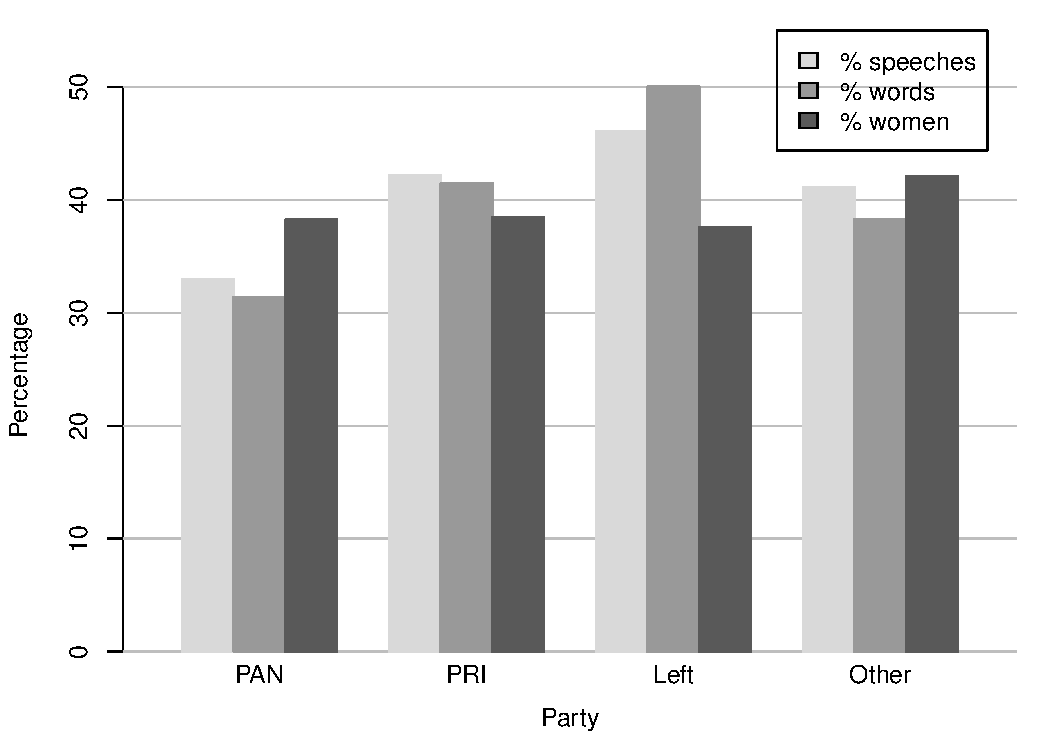
\includegraphics[width=.67\columnwidth]{../plots/women-bar.pdf}
\singlespacing
\begin{scriptsize}
\begin{verbatim}
(Data to do the gender barchart in Stata is this.)
     party pct.women pct.speech pct.words
   1   pan     38.25      32.94     31.39
   2   pri     38.44      42.15     41.47
   3  left     37.61      46.06     50.03
   4 other     42.06      41.13     38.29
   5 total     38.65      41.18     40.76
\end{verbatim}
\end{scriptsize}
\doublespacing
    \caption{Gender and speechmaking by party}\label{F:women}
\end{figure}

Figure \ref{F:women} shows the percentage of debate by female members, pooled across the terms observed, and broken by main parties. Light gray bars are speeches by female deputies, mid gray bars the total words delivered by female deputies, and dark gray bars the percentage of women in the legislative party across terms observed. Relating speech and numerical importance shows that the average woman deputy from the left spoke 63 percent more words overall than their male counterparts. The reverse relation holds among PAN deputies but much less acute. The other parties break more or less even. In general, gender differences between parties are mild. 

Single-term limits offer little leverage to evaluate seniority effects on floor access. Members wishing to return had to wait one term at least. It is remarkable that, despite this, 14 percent of members had previous federal deputy experience. A hint that the removal of single-terms will not be shunned by lack of static ambition (as in Argentina, for instance). Freshmen spoke 1122 words per period on average, compared to 2019 for members with past terms in Congress. Member-periods with one past term made 44 percent more speeches and spoke 68 percent more words than those with none; with two past terms instead of one, 30 percent more speeches and 48 percent more words; but those with more than two past terms gave 33 percent less speeches and 53 percent fewer words than those with two. This drop could be attributable to earlier recruitment of senior members, antedating competitive politics; or it could be due to higher likelihood that senior members occupy positions that might depress willingness to speak despite floor access possibilities. The multivariate analysis might shed some light.  

\begin{table}
  \begin{scriptsize}
    \begin{verbatim}
(Data to do the seniority barchart in Stata is this.)
|------------+-------------+-------------+----------------+----------------|
|            | Mean number | Mean number |                |                |
|            | of speeches | of speeches | Member-periods | Member-periods |
| Past terms |       women |         men |          women |            men |
|------------+-------------+-------------+----------------+----------------|
|          0 |        1.94 |        1.69 |           3015 |           4944 |
|         >0 |        2.95 |        2.57 |            610 |           1409 |
|          1 |        3.02 |        2.36 |            483 |           1102 |
|          2 |        2.74 |        3.66 |            115 |            229 |
|         3+ |        1.92 |        2.36 |             12 |             78 |
|------------+-------------+-------------+----------------+----------------|
    \end{verbatim}
  \end{scriptsize}
\caption{Seniority and floor access, member-periods}
\end{table}
  
To analyze participation in floor debates, I fit multivariate regression models to words spoken. In the right side are status variables, member characteristics, and controls. Units are member-periods. 

/Status variables/ A dummy for *majority* status indicates members from Morena in the 64th Legislature---the only party controlling over 50 percent of seats. If debate is an (imperfect) substitute for legislative outcomes, then minority members demand more frequent floor participation \citep{proksch-slapin2015book}. On the contrary, if members put value on debate per se, the majority may demand it as much as others, possibly with better access to the floor. Next, a dummy for committee *chair* status. When producing a report, the chair has privileged access to the floor, and this should translate into more speech. A dummy for party *leader* status completes this set. Leaders allocate party speakers. Whether or not they take advantage of this privilege remains an open question, a good leader ought to distribute the goodies, or risk removal. 

/Member variables/ Aside from *woman* and *seniority*, regressors in this group include *smd*, a dummy equal one for members elected in single-member districts. Systematic differences in members' pork requests are attributable to the method of election \citep{kerevelPork2015}, which may also translate into higher demand for access to the floor. I also interact this regressor with a dummy indicating the 64th Legislature, which dropped single-term limits (*smd x reelection*). The more personal vote should generate higher demand for floor access. *Party size* is the percentage of seats the member's party holds. Larger parties must divide the slot that all parties get to take the floor among more members, and this should show up as a negative regression coefficient. And a dummy *suplente* controls for substitute members. Regressors not in the right side include members' ages due to incomplete data, and party ideology, which made no difference in the estimates.

/Other controls/ Also in the right side are dummies for the *62nd* and *64th* terms (the 60th is the baseline) and another for *extraordinary* periods. Finally, with the option to take leaves of absence and have suplentes take over, some members served incomplete periods. The *exposure* is a member's tenure, the number of days served in the period, logged. Higher exposure offers more opportunities for floor access. Unlike other chapters, models exclude party fixed effects, they made no substantive difference in the estimates reported.

Table \ref{T:regs} reports the estimation of six different model specifications. In the left side are both flavors of the dependent variable. Count models of speeches were fit with negative binomial regression (1 and 2) and zero-inflated poisson regression (3), while models of words relative to tenure with ordinary least squares (4, 5, and 6). Specifications vary the regressors. Models 2, 3, 5, and 6 include fixed term effects to capture any heterogeneity between Legislatures that are pooled together. Model 6 also estimates separate error terms for each member, intended to capture individual heterogeneity. And model 3 accounts for the excess of zeroes in the distribution. The overall fit is correct across models, likelihood ratio tests (not reported) reject the intercept-only model with much confidence.


\begin{table} \centering 
  \begin{tiny}
\begin{verbatim}
Regression results
============================================================================================================================
                               DV = Speeches in period                           DV = Words/exposure in period           
                   ----------------------------------------------     ---------------------------------------------------
                         (1)            (2)            (3)                (4)                  (5)                 (6)       
---------------------------------------------------------------------------------------------------------------------------
Exposure (logged)      0.99***        1.32***        1.07***                                                               
                        (0.02)         (0.04)        (0.04)                                                                
                                                                                                                           
Majority               1.20***        0.98***        1.11***           826.87***           1,738.55***         1,102.46*** 
                        (0.05)         (0.06)        (0.04)             (84.75)             (128.10)            (219.25)   
                                                                                                                           
Party leader           0.35***        0.31***        0.22***          2,241.56***          1,911.89***         1,260.70*** 
                        (0.08)         (0.08)        (0.04)             (202.81)            (199.88)            (302.50)   
                                                                                                                           
Comm. chair            0.28***        0.26***        0.12***           289.72***            225.24***            184.63    
                        (0.04)         (0.03)        (0.02)             (78.23)              (76.64)            (127.37)   
                                                                                                                           
Seniority              0.11***        0.12***        0.10***           210.68***            245.54***           253.18***  
                        (0.02)         (0.02)        (0.01)             (46.37)              (45.33)             (83.10)   
                                                                                                                           
Woman                  0.13***        0.09***        0.04**            136.54***            125.68**              16.18    
                        (0.02)         (0.02)        (0.02)             (52.64)              (52.14)             (96.83)   
                                                                                                                           
Party size             -0.05***       -0.04***      -0.04***           -61.52***            -71.85***           -63.13***  
                       (0.001)        (0.001)        (0.001)             (1.92)              (2.20)              (3.76)    
                                                                                                                           
SMD                      0.03          -0.06*         -0.01              -48.69              -90.05              -113.31   
                        (0.03)         (0.03)        (0.02)             (53.48)              (63.34)            (112.33)   
                                                                                                                           
SMD x reelect                         0.26***        0.10***                                232.39**              -8.32    
                                       (0.05)        (0.03)                                 (111.13)            (182.94)   
                                                                                                                           
Suplente               -0.17***        -0.09        -0.23***           -271.52**           -346.94***           -330.99**  
                        (0.06)         (0.06)        (0.05)             (106.35)            (103.79)            (137.19)   
                                                                                                                           
62nd Leg.                             0.25***        0.24***                                726.90***           843.14***  
                                       (0.03)        (0.02)                                  (60.94)             (94.39)   
                                                                                                                           
64th Leg.                             0.17***        0.16***                               -279.10***           316.26**   
                                       (0.05)        (0.03)                                 (107.10)            (158.53)   
                                                                                                                           
Extraordinary                         0.67***        0.69***                              -1,234.16***        -1,240.27*** 
                                       (0.08)        (0.07)                                  (64.62)             (43.42)   
                                                                                                                           
Constant               -1.66***       -2.97***      -1.95***          2,874.07***          3,064.88***         2,805.63*** 
                        (0.08)         (0.15)        (0.13)             (68.55)              (84.01)            (140.25)   
                                                                                                                           
---------------------------------------------------------------------------------------------------------------------------
Fixed effects             no            term           term                no                term                term      
Random effects            no             no             no                 no                  no                member     
Estimation method      negative       negative    zero-inflated           OLS                 OLS                linear     
                       binomial       binomial       poisson                                                  mixed-effects 
---------------------------------------------------------------------------------------------------------------------------
theta                  1.55*** (0.05)   1.65*** (0.05)                                                                   
---------------------------------------------------------------------------------------------------------------------------
Observations            9,978          9,978          9,978              9,978                9,978               9,978    
R2                                                                        0.14                0.18                         
Akaike Inf. Crit.     32,689.90      32,478.98     34,832.82                                                   178,880.70  
===========================================================================================================================
Note:                                                                                                *p<0.1; **p<0.05; ***p<0.01
\end{verbatim}
  \end{tiny}
  \caption{Models of legislative debate (standard errors in parentheses)} 
  \label{T:regs} 
\end{table} 

%Adjusted R2                   0.15                     0.18                                                                     
%Log Likelihood                                                          -85,188.83     -16,232.18     -16,126.53    -17,305.06 
%Bayesian Inf. Crit.                                                     170,515.00                                              
%Residual Std. Error   2,504.36 (df = 9485)     2,465.37 (df = 9481)                                                             
%F Statistic         210.29*** (df = 8; 9485) 170.19*** (df = 12; 9481)                                                          

Interesting patterns emerge from coefficient estimates. Party size exerted a negative and statistically significant effect in member floor access across specifications. This is easier to interpret from OLS coefficients: other variables constant, changing the party size from large (40 percent of seats) to small (15 percent) associates with a predicted drop of 1,650 words per member in the period. Martin Luther King took 16 minutes to deliver his famous "I have a dream" speech, which approximates that word count. I also find a positive, large, and statistically significant effect of majority status, which acts against size. Far from letting legislative accomplishments speak for themselves, majority members take the floor systematically more than those of similar-sized parties. Figure \ref{F:predict} demonstrates the discontinuity through simulation with model 2 parameters. As party size crosses the majority threshold the member gets a bonus, delivering a number of speeches comparable to a party with 25 to 30 percent of seats.

%Note that the relative equals absolute words divided by the share of period p's duration that member i served, so the *exposure* is in the left side of OLS models and not in the right. 
%*words(i,p) x days(p)  / exposure(i,p)*

Other forms of status also associate positively to floor access, with results somewhat sensitive to model specification. Party leadership exerts a substantially larger effect than majority status on speech length, but much smaller on the number of speeches. Leaders get privileged floor access and appear to specialize in longer speeches, probably on more significant legislation. Committee chairs also deliver more speeches than other members, but controlling for term and member effects bears upon OLS coefficient significance, both substantially and statistically, hinting to important differences in speech length across committee jurisdictions and individuals.

I also find positive effects of seniority and gender that resonate with the bivariate patterns of floor access. The coefficient for *women* is not robust to random member effects (accounting for zero-inflation also bears on impact). This is probably due to the concentration of debate by women highlighted above, some deputies taking the floor disproportionately more than others. Overall, the effect of gender appears to be on par with that of one additional term of seniority in Figure \ref{F:avgmgeff}, which reports average marginal effects.

\begin{figure}
  \centering
    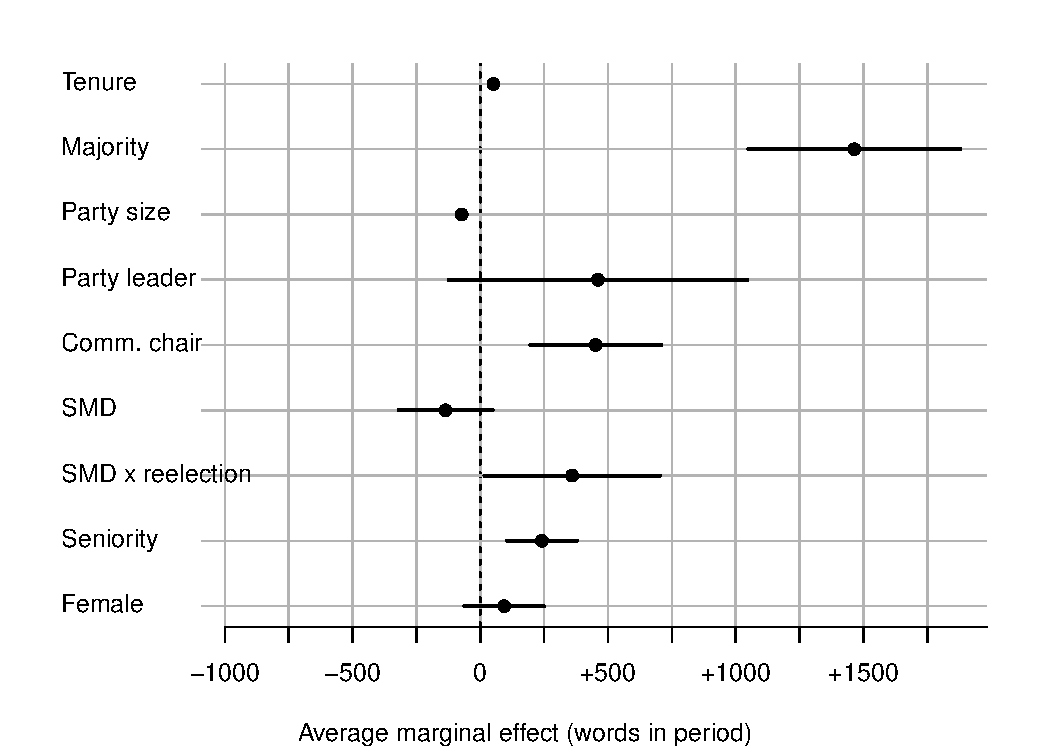
\includegraphics[width=.67\columnwidth]{../plots/avgMgEffects.pdf}
    \caption{Average marginal effects from model 2. Circles report the effect in the expected number of speeches per period of a unit change in each independent variable, all else at mean values; bars are 95-percent confidence intervals.}\label{F:avgmgeff}
\end{figure}

\singlespacing
\begin{scriptsize}
\begin{verbatim}
(Data to prepare the average marginal effects plot in stata. Lower and upper are 95-pct ci limits)
                       factor     AME     SE        z      p   lower   upper
            Tenure (exposure)  0.1029 0.0032  32.0872 0.0000  0.0967  0.1092
                     Majority  1.9258 0.1256  15.3299 0.0000  1.6796  2.1720
                 Party leader  0.6200 0.1543   4.0181 0.0001  0.3176  0.9224
                  Comm. chair  0.5110 0.0686   7.4456 0.0000  0.3765  0.6455
               Previous terms  0.2298 0.0394   5.8267 0.0000  0.1525  0.3071
                        Woman  0.1705 0.0493   3.4615 0.0005  0.0740  0.2670
                   Party size -0.0857 0.0025 -33.6091 0.0000 -0.0907 -0.0807
                          SMD -0.1129 0.0592  -1.9074 0.0565 -0.2290  0.0031
             SMD x reelection  0.5032 0.1053   4.7774 0.0000  0.2967  0.7096
      Suplente (not reported) -0.1820 0.1170  -1.5553 0.1199 -0.4113  0.0473
     62nd Leg. (not reported)  0.4859 0.0582   8.3514 0.0000  0.3719  0.5999
     64th Leg. (not reported)  0.3445 0.0952   3.6165 0.0003  0.1578  0.5311
 Extraordinary (not reported)  1.3190 0.1559   8.4624 0.0000  1.0135  1.6245
\end{verbatim}
\end{scriptsize}
\doublespacing


A null finding of interest involves the method of election. The coefficient for *smd* is indistinguishable from zero across models. Average marginal effects aid in negative binomial regression coefficient interpretation: in contrast to PR members and holding all other regressors at their mean, deputies elected in SMDs spoke slightly less, about 125 words in the period; the 95-percent confidence interval, however, barely excludes the zero and this signal therefore could be the product of chance alone. But look at the change in slope when interacted with reelection: this marginal effect is not just positive, but sufficient to cancel the negative pull of SMDs. Now a signal is discernible from random noise, even after controlling for majority status (the other big change in the 64th Legislature). Figure \ref{F:predict} makes this effect plain, a gap separates confidence intervals of predicted speeches by SMD members who can reelect (darker) and the term-limited (lighter). This finding hints to the invigoration of the personal vote after the removal of term limits and is worthy of more careful examination. 

\begin{figure}
  \centering
    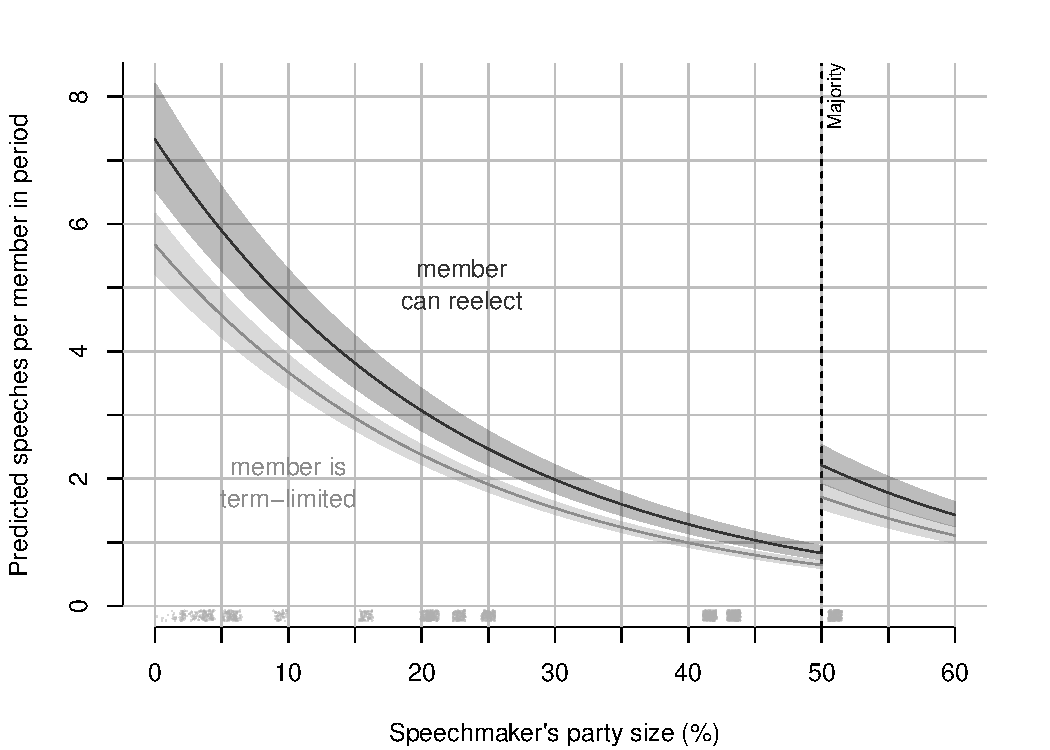
\includegraphics[width=.67\columnwidth]{../plots/predictedWords.pdf}
    \caption{Predicted number of speeches by party size. Lines report point predictions using model 2, bands are 95-percent confidence intervals. Miniature points above the x-axis are observed members' party sizes (x- and y-jittered for visibility).}\label{F:predict}
\end{figure}

\emm{Please advise on the style of the book for this plot, I could not figure it out from the email.}


\section{Informal waterproofing} % [ca 1000 words]

Where do the Cámara's debate institutions sit relative to other stylized assemblies? Figure \ref{F:comparison} does a simple comparative exercise by intersecting the permeability of floor access and the degree of informality in the constraints adopted.

\begin{figure}
  \centering
    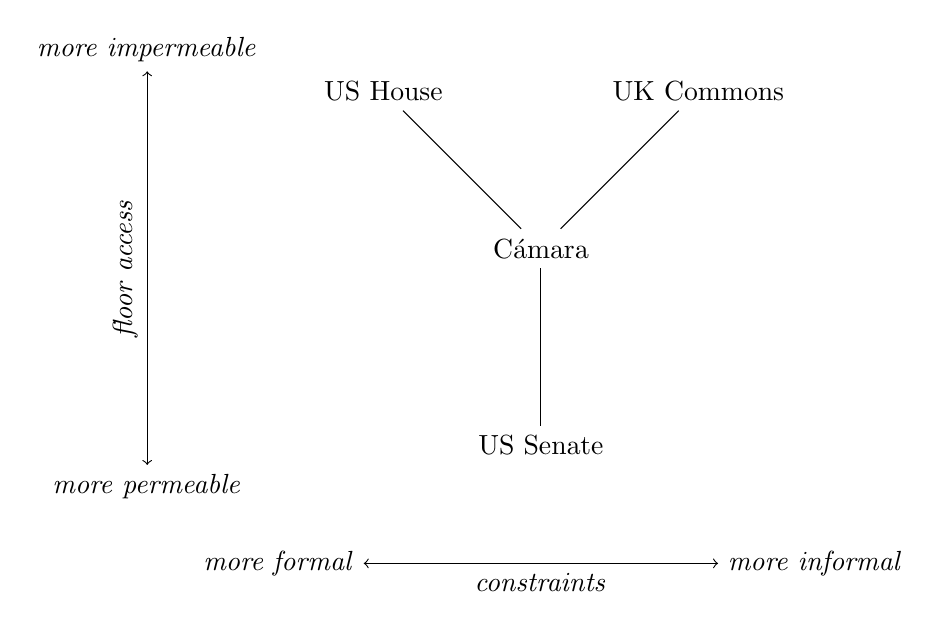
\begin{tikzpicture}
      \node at (-2, 2) {US House};
      \node at ( 2, 2) {UK Commons};
      \node at ( 0, 0) {Cámara};
      \node at ( 0,-2.5) {US Senate};
      \draw (-.25, .25) -- (-1.75, 1.75);
      \draw ( .25, .25) -- ( 1.75, 1.75);
      \draw (0,   -.25) -- ( 0,   -2.25);
      \draw[<->] (-2.25,-4) node[left] {\emph{more formal}} -- node[below] {\emph{constraints}} (2.25,-4) node[right] {\emph{more informal}};
      \draw[<->] (-5,-2.75) node[below] {\emph{more permeable}} -- node[sloped,above] {\emph{floor access}} (-5,2.25) node[above] {\emph{more impermeable}};
%      \draw[<->] (-5,-2.75) node[below] {\emph{less restrictive}} -- (-5,2.25) node[above] {\emph{more restrictive}};
    \end{tikzpicture}  
\caption{Formal and informal restrictions to members' legislative rights}\label{F:comparison}
\end{figure}

Make the Cámara less permeable and more informal, get the U.K. House of Commons. As plenary time became a scarce commodity with suffrage extension and industrialization, British private members gradually abdicated their parliamentary rights, delegating all-encompassing legislative authority to the cabinet \citep{cox.1987}. But speaking time in the Commons remains formally reserved for individual MPs, who are recognized by a non-partisan Speaker (Blumenau and Damiani in this volume). Therefore the efficient secret of British politics that turned backbenchers into legislative nonentities by the mid-1880s was and remains an informal arrangement, a superimposition of party hierarchy over formal procedure. Disruption of the party system inevitably reinstates formal member prerogatives, to some extent at least. To the cabinet ministers' dismay, the Brexit section that split both parties since the 2016 referendum resurrected many of the Speaker's agenda-setting powers that had been dormant for decades---if not centuries \citep{economist-bercow.2019}.

Make less permeable but more formal, get the U.S. House. The adoption of Reed's rules in the 1880s achieved much the same centralization of agenda power as in Commons---allowing the Speaker to curb the minority's power to delay and to select what bills to consider in what order \citep{denhartog.2004phd,cox.mccubbins.2005}. Particular to debate, the crucial innovation empowered the Speaker to refuse to recognize members seeking to make dilatory motions, making floor access impermeable. Unlike Commons, however, the House has routinely written these constraints in the rules it adopts every two years at the start of each term.  

Last, add permeability while keeping informality more or less constant, get the U.S. Senate. Cloture to stop debate requires three-fifth of Senate floor support, against majority for the Cámara's previous question (Gelman and Goplerud, this volume). After a committee reports out a bill, it is automatically included in the calendar, as in the Cámara. However, by precedent, the majority leader, in consultation with the minority leader, schedules what bill in the calendar shall be considered next \citep{roberts-smith.2007,campbell.cox.mccubbins.2002}. Absent this /informal/ rule, the leader's negative agenda power would be severely weakened and ineffective.

Why so many assemblies weaken members' legislative rights through informal mechanisms, but retain those rights formally in place is an interesting puzzle. The central intuition in Riker's work offers a clue: every majority is the sum of minorities. There is no guarantee that the tide won't turn in the near future, majorities losing elections or splitting to become minorities. Retaining members' formal rights in place is an insurance policy to remain somewhat relevant when all else fails. \citet{wawro.schickler.filibuster.2007} document routine threats to "go nuclear" and remove minority rights in today's polarized Senate, yet the filibuster remains firmly in place.


%% - One difficulty = changing Reglamento requires two-thirds vote. 
%% - Tomas de tribuna
%% - suspension of rules by Conferencia typified only for discharge, two-thirds. Art 77 cpeum. 
%% - Presiding officer can summon public force to restore order, but in practice never used. 
%% - Can kill the mike, but others can raise their voices
%% 4. Para atender una situación no prevista en el Reglamento, el Presidente podrá dictar una resolución de carácter general, siempre que haya la opinión favorable de la Mesa Directiva y de la Junta. En caso contrario, este tipo de resoluciones sólo tendrán efecto con la aprobación de la mayoría simple del Pleno.


\section{Conclusion} % [ca 500 words]

Tension lies at the heart of legislative debate in the Cámara. On one hand, parties have informally, but effectively managed to reign in members' capacity to take the floor. The effects that the chapter's regression models uncovered for the majority, for leaders, and for committee chairs are all channeled through party structures in the Junta. On the other hand, formal rules grant individual members rights of recognition to take the floor and, we have seen, these take many guises. The effect attributable to SMDs after the removal of term limits is, in all likelihood, associated to renovated personal vote incentives that members face. 

Whether or not the informal solution to avoid plenary bottlenecks continues to operate as it has so far in the Cámara is uncertain. Little intra-party competition used to remove personal vote incentives that leads members to differentiate by taking the floor in Proksch and Slapin's model. With the removal of term limits, incumbents with static ambition may soon start overwhelming the system by exploiting the formal autonomy of floor debate in their need to strengthen their electoral connection.

It is important to keep in mind that the place of debate in the legislative process is /after/ negative agenda filters. Agenda-setting lets leaders prevent consideration of motions when they anticipate debate to go in undesired directions---speakers opening issues that threaten to divide the majority. When and if parties can no longer prevent delays as they have, pressure to reform the rules will inevitably build up. Reform could give leaders strong ex-ante vetoes to prevent moving unwanted bills to the floor, precluding debate; by removing the formal rights that render floor access so permeable; or both. 

%But secondary is not the same as unimportant. Position taking is a central activity in electoral connection \citep{mayhew.1974} and home style \citep{fenno.1978} models of political ambition. And plenary debate is the chief position taking tool in the chamber. 

%Proksch and Slapin theorize that personal vote incentives make legislators organize the assembly with high levels of autonomy in floor debate. 

%With little intra-party competition, such incentives are low in Mexico, but they are bound to increase due to the removal of single-term limits. 

%The collapse of the three-party system in 2018 also plays against. Perhaps the heterogeneous coalition that gave Morena unified control of government will manage to consolidate, imposing a new informal arrangement, in spite of the 2020 covid depression.

%% - A Legislature (with Roman numerals for reasons I ignore) is an elected chamber for a legislative term, called a Congress in the U.S. Concurrent with presidential elections the chamber of deputies renovates in whole, and again at the presidential mid-term. Diputados remain three years in office and were single term-limited up to 2021. The 2021 mid-term election will be the first since 1932 to allow incumbents on the ballot, a major change in Mexican legislative politics.
%% - Legislative years break into two "ordinary periods", one covering the months of September through December, inclusive, another February through April, also inclusive. "Extraordinary periods" may be convened during the recess in order to consider a specific bill. Analysis aggregates each member's speeches in the duration of a given period (merging together all extraordinary periods that year, if any). So members in a legislative year like 2012-13 (that had no extraordinary periods) have two word aggregates in the dataset, one for each ordinary period; in a year like 2013-14 (that did), they have three word aggregates in the data. Periods are the units of aggregation in the analysis. 
%% - A plenary session is a specific date in the calendar when diputados met. During ordinary periods, sessions are usually held on Tuesdays and Thursdays, and may be scheduled in other weekdays if the Jucopo so decides. Diputados met on forty and thirty-one days in the first and second ordinary periods of 2013-14, respectively, and nine days in extraordinary periods, for a yearly total of eighty session days. (A session in North-American legislative parlance is a Mexican period.)


%\listofendnotes

\newpage

\singlespacing

\bibliographystyle{apsr}

%\bibliography{../bib/magar}

\begin{thebibliography}{xx}

\subsection*{Software libraries}

\harvarditem[Bates et~al.]{Bates, M{\"a}chler, Bolker \harvardand\
  Walker}{2015}{r.lme4}
Bates, Douglas, Martin M{\"a}chler, Ben Bolker \harvardand\ Steve Walker. 2015.
\newblock ``Fitting Linear Mixed-Effects Models Using {lme4}.'' {\em Journal of
  Statistical Software} 67(1):1--48.

\harvarditem{Grolemund \harvardand\ Wickham}{2011}{r.lubridate}
Grolemund, Garrett \harvardand\ Hadley Wickham. 2011.
\newblock ``Dates and Times Made Easy with {lubridate}.'' {\em Journal of
  Statistical Software} 40(3):1--25.

\harvarditem{Hlavac}{2018}{r.stargazer}
Hlavac, Marek. 2018.
\newblock {\em stargazer: Well-Formatted Regression and Summary Statistics
  Tables}.
\newblock Bratislava, Slovakia:  Central European Labour Studies Institute
  (CELSI).
\newblock R package version 5.2.2.

\harvarditem{Leeper}{2018}{r.margins}
Leeper, Thomas~J. 2018.
\newblock {\em margins: Marginal Effects for Model Objects}.
\newblock R package version 0.3.23.

\harvarditem{{R Dev.\ Core Team}}{2011}{r.cite}
{R Dev.\ Core Team}. 2011.
\newblock ``R: A Language and Environment for Statistical Computing.'' R
  Foundation for Statistical Computing \url{http://www.R-project.org}.

\harvarditem{Venables \harvardand\ Ripley}{2002}{r.mass}
Venables, W.~N. \harvardand\ B.~D. Ripley. 2002.
\newblock {\em Modern Applied Statistics with S}.
\newblock Fourth ed. New York:  Springer.
\newblock ISBN 0-387-95457-0.

\harvarditem{Wickham}{2011}{r.plyr}
Wickham, Hadley. 2011.
\newblock ``The Split-Apply-Combine Strategy for Data Analysis.'' {\em Journal
  of Statistical Software} 40(1):1--29.

\harvarditem{Zeileis \harvardand\ Grothendieck}{2005}{r.zoo}
Zeileis, Achim \harvardand\ Gabor Grothendieck. 2005.
\newblock ``zoo: S3 Infrastructure for Regular and Irregular Time Series.''
  {\em Journal of Statistical Software} 14(6):1--27.

\subsection*{Statutes}

\harvarditem{Org\'anica}{2019}{loceum.2019}
Org\'anica. 2019.
\newblock ``Ley Org\'anica del Congreso de los Estados Unidos Mexicanos (last
  modified 8 May 2019).'' Secretar\'ia de Servicios Parlamentarios
  \url{http://www.diputados.gob.mx/LeyesBiblio/marco.htm} (visited 10 Jun.
  2020).

\harvarditem{Reglamento}{2019}{reglamentoDipMx.2019}
Reglamento. 2019.
\newblock ``Reglamento de la C\'amara de Diputados (last modified 18 Dec.\
  2019).'' Secretar\'ia de Servicios Parlamentarios
  \url{http://www.diputados.gob.mx/LeyesBiblio/marco.htm} (visited 10 Jun.
  2020).

\subsection*{Books, articles, and newspapers}
  
\harvarditem{Ascencio \harvardand\
  Kerevel}{2021}{ascencio.kerevel.cand-sel-beh.2021}
Ascencio, Sergio~J. \harvardand\ Yann~P. Kerevel. 2021.
\newblock ``Party Strategy, Candidate Selection, and Legislative Behavior in
  {M}exico.'' {\em Legislative Studies Quarterly} forthcoming(tba).

\harvarditem{B{\'e}jar~Algazi}{2012}{bejarQuienLegisla2012}
B{\'e}jar~Algazi, Luisa. 2012.
\newblock ``?`{Q}ui\'en legisla en {M\'e}xico? {D}escentralizaci\'on y proceso
  legislativo.'' {\em Revista Mexicana de Sociolog\'ia} 74(4):619--47.

\harvarditem{B{\'e}jar~Algazi}{2009}{bejar.Comisiones2009ed.book}
B{\'e}jar~Algazi, Luisa, ed. 2009.
\newblock {\em Qu\'e hacen los legisladores en M\'exico: El trabajo en
  comisiones}.
\newblock {M\'e}xico City:  FCPyS–UNAM/Miguel Angel Porr\'ua.

\harvarditem[Cain, Ferejohn \harvardand\ Fiorina]{Cain, Ferejohn \harvardand\
  Fiorina}{1987}{cain.etal.1987}
Cain, Bruce~E., John~A. Ferejohn \harvardand\ Morris~P. Fiorina. 1987.
\newblock {\em The personal vote: constituency service and electoral
  independence}.
\newblock Cambridge, MA:  Harvard University Press.

\harvarditem[Campbell, Cox \harvardand\ McCubbins]{Campbell, Cox \harvardand\
  McCubbins}{2002}{campbell.cox.mccubbins.2002}
Campbell, Andrea~C., Gary~W. Cox \harvardand\ Mathew~D. McCubbins. 2002.
\newblock Agenda Power in the {US} {S}enate, 1877--1986.  In {\em Party,
  Process, and Political Change in Congress: New Perspectives on the History of
  Congress}, ed. David~W. Brady \harvardand\ Mathew~D. McCubbins.
\newblock Palo Alto:  Stanford University Press.

\harvarditem{Carey \harvardand\ Shugart}{1995}{carey.shugart.1995}
Carey, John~M. \harvardand\ Matthew~S. Shugart. 1995.
\newblock ``Incentives to Cultivate a Personal Vote: A Rank Ordering of
  Electoral Formulas.'' {\em Electoral Studies} 14(4):417--39.

\harvarditem{Casar}{2011}{casar.2011}
Casar, Mar\'ia~Amparo. 2011.
\newblock ``?`C\'omo y cu\'anto gasta la {C\'a}mara de {D}iputados?'' CIDE,
  cuaderno de debate 8.

\harvarditem{Casar}{2016}{casar.agsetting.2016}
Casar, Mar\'ia~Amparo. 2016.
\newblock Parliamentary agenda setting in {L}atin {A}merica: The case of
  {M}exico.  In {\em Legislative Institutions and Lawmaking in {L}atin
  {A}merica}, ed. Eduardo Alem\'an \harvardand\ George Tsebelis.
\newblock Oxford University Press pp.~148--74.

\harvarditem{Casar \harvardand\ Marv\'an~Laborde}{2014}{casar.marvan2014book}
Casar, Mar\'ia~Amparo \harvardand\ Ignacio Marv\'an~Laborde, eds. 2014.
\newblock {\em Reformar sin mayor\'ias: La din\'amica del cambio constitucional
  en {M}\'exico, 1997--2012}.
\newblock {M}exico City:  Taurus.

\harvarditem{Cornelius}{1996}{cornelius.1996}
Cornelius, Wayne~A. 1996.
\newblock {\em Mexican Politics in Transition: The Breakdown of a
  One-Party-Dominant Regime}.
\newblock La Jolla, CA:  Center for U.S.--Mexican Studies.

\harvarditem{Cos\'io~Villegas}{1981}{cosio.villegas.1981}
Cos\'io~Villegas, Daniel. 1981.
\newblock {\em El sistema pol\'itico mexicano}.
\newblock {M}exico City:  Joaqu\'in Mortiz.

\harvarditem{Cox}{1987}{cox.1987}
Cox, Gary~W. 1987.
\newblock {\em The Efficient Secret: The Cabinet and the Development of
  Political Parties in {V}ictorian {E}ngland}.
\newblock New York:  Cambridge University Press.

\harvarditem{Cox}{2006}{cox.2006}
Cox, Gary~W. 2006.
\newblock The Organization of Democratic Legislatures.  In {\em The Oxford
  Handbook of Political Economy}, ed. Barry~R. Weingast \harvardand\ Donald~A.
  Wittman.
\newblock New York:  Oxford University Press pp.~141--61.

\harvarditem{Cox \harvardand\ McCubbins}{1993}{cox.mccubbins.1993}
Cox, Gary~W. \harvardand\ Mathew~D. McCubbins. 1993.
\newblock {\em Legislative {L}eviathan: Party Government in the {H}ouse}.
\newblock Berkeley:  University of California Press.

\harvarditem{Cox \harvardand\ McCubbins}{2005}{cox.mccubbins.2005}
Cox, Gary~W. \harvardand\ Mathew~D. McCubbins. 2005.
\newblock {\em Setting the Agenda: Responsible Party Government in the {US}
  {H}ouse of {R}epresentatives}.
\newblock New York:  Cambridge University Press.

\harvarditem{Den~Hartog}{2004}{denhartog.2004phd}
Den~Hartog, Christopher~F. 2004.
\newblock Limited Party Government and the Majority Party Revolution in the
  Nineteenth-Century {H}ouse PhD thesis UCSD.

\harvarditem[D\'iaz~Cayeros, Est\'evez \harvardand\ Magaloni]{D\'iaz~Cayeros,
  Est\'evez \harvardand\
  Magaloni}{2016}{diaz-estevez-magaloni-Poverty-book.2016}
D\'iaz~Cayeros, Alberto, Federico Est\'evez \harvardand\ Beatriz Magaloni.
  2016.
\newblock {\em The Political Logic of Poverty Relief: Electoral Strategies and
  Social Policy in {M}exico}.
\newblock New York:  Cambridge University Press.

\harvarditem{Dion \harvardand\ Huber}{1996}{dion.huber.1996}
Dion, Douglas \harvardand\ John~D. Huber. 1996.
\newblock ``Procedural Choice and the {H}ouse Committee on Rules.'' {\em The
  Journal of Politics} 58(1):25--53.

\harvarditem{Economist}{2019}{economist-bercow.2019}
Economist, The. 2019.
\newblock ``John {B}ercow, speaker of the asylum.'' Bagehot, January 10th.

\harvarditem{Enr\'iquez~Gonz\'alez}{2018}{enriquez-dinastias2018itam}
Enr\'iquez~Gonz\'alez, Jos\'e~Ram\'on. 2018.
\newblock Dinast\'ias pol\'iticas municipales en M\'exico B.a. thesis Intituto
  Tecnol\'ogico Aut\'onomo de M\'exico.

\harvarditem{Heller \harvardand\ Weldon}{2003}{heller.weldon.2003}
Heller, William~B. \harvardand\ Jeffrey~A. Weldon. 2003.
\newblock Reglas de votaci\'on y la estabilidad en la C\'amara de Diputados.
  In {\em El Congreso Mexicano despu\'es de la alternancia}, ed. Luisa
  B\'ejar~Algazi \harvardand\ Rosa~Mar\'ia Mir\'on~Lince.
\newblock {M}exico {C}ity:  Asociaci\'on Mexicana de Estudios Parlamentarios
  and Instituto de Investigaciones Legislativas del Senado de la Rep\'ublica
  pp.~85--119.

\harvarditem{Jacobson}{1997}{jacobson.1997}
Jacobson, Gary~C. 1997.
\newblock {\em The Politics of Congressional Elections}.
\newblock 4$^{th}$ ed. New York:  Longman.

\harvarditem{Kerevell}{2015}{kerevelPork2015}
Kerevell, Yann~P. 2015.
\newblock ``Pork-barreling without reelection? Evidence from the {M}exican
  {C}ongress.'' {\em Legislative Studies Quarterly} 40:137--66.

\harvarditem{Langston}{2008}{langston.2008}
Langston, Joy. 2008.
\newblock Legislative recruitment in {M}exico.  In {\em Pathways to Power:
  Political Recruitment and Democracy in Latin America}, ed. Peter Siavelis
  \harvardand\ Scott Morgenstern.
\newblock Penn State University Press.

\harvarditem{L\'opez~Lara}{2013}{lopez.lara.aldf2013}
L\'opez~Lara, Alvaro~F. 2013.
\newblock Ideolog\'ia y coaliciones en la {A}samblea {L}egislativa del
  {D}istrito {F}ederal.  In {\em ?`Qui\'en, c\'omo y qu\'e se legisla en
  {M\'e}xico?}, ed. Luisa B\'ejar~Algazi.
\newblock {M}exico City:  UNAM pp.~217--64.

\harvarditem{Lujambio}{1996}{lujambio.1996}
Lujambio, Alonso. 1996.
\newblock {\em Federalismo y Congreso en el cambio pol\'itico de {M\'e}xico}.
\newblock {M}exico City:  Universidad Nacional Aut\'onoma de {M\'e}xico.

\harvarditem{Magar}{2017}{magarInstReel.2017}
Magar, Eric. 2017.
\newblock ``Consecutive reelection institutions and electoral calendars since
  1994 in {M}exico V2.0.'' \url{http://dx.doi.org/10.7910/DVN/X2IDWS}, Harvard
  Dataverse [distributor].

\harvarditem[Magar et~al.]{Magar, Trelles, Altman \harvardand\
  McDonald}{2016}{magar.altman.mcd.trelles2016pg}
Magar, Eric, Alejandro Trelles, Micah Altman \harvardand\ Michael~P. McDonald.
  2016.
\newblock ``Components of partisan bias originating from single-member
  districts in multi-party systems: An application to {M}exico.'' {\em
  Political Geography} 57(1):1--12.

\harvarditem{Molinar}{1991}{molinar.1991a}
Molinar, Juan. 1991.
\newblock {\em El tiempo de la legitimidad: elecciones, autoritarismo y
  democracia en {M\'e}xico}.
\newblock {M}exico City:  Cal y arena.

\harvarditem{Moreno}{2009}{moreno.decisElec.2009}
Moreno, Alejandro. 2009.
\newblock {\em La decisi\'on electoral: votantes, partidos y democracia en
  {M\'e}xico}.
\newblock {M}exico City:  Porr\'ua.

\harvarditem{Piscopo}{2016}{piscopo.2016}
Piscopo, Jennifer~M. 2016.
\newblock ``When Informality Advantages Women: Quota Networks, Electoral Rules
  and Candidate Selection in Mexico.'' {\em Government and Opposition}
  51(3):487--–512.

\harvarditem{Poir\'e}{2002}{poire.phd.2002}
Poir\'e, Alejandro. 2002.
\newblock Bounded ambitions. Party nominations, discipline, and defection:
  {M}exico's PRI in comparative perspective PhD thesis Dept. of Government,
  Harvard University.

\harvarditem{Prata}{2001}{prata.2006}
Prata, Adriana. 2001.
\newblock A Study of Party Discipline and Agenda Control in National
  Legislatures Ph{D}. dissertation University of California, San Diego.

\harvarditem{Proksch \harvardand\ Slapin}{2015}{proksch-slapin2015book}
Proksch, Sven-Oliver \harvardand\ Jonathan~B. Slapin. 2015.
\newblock {\em The Politics of Parliamentary Debate: {P}arties, Rebels and
  Representation}.
\newblock Cambridge University Press.

\harvarditem{Roberts \harvardand\ Smith}{2007}{roberts-smith.2007}
Roberts, Jason~M. \harvardand\ Steven~S. Smith. 2007.
\newblock The Evolution of Agenda-Setting Institutions in {C}ongress: Path
  Dependency in {H}ouse and {S}enate Institutional Development.  In {\em Party,
  Process, and Political Change in Congress Volume 2: Further New Perspectives
  on the History of Congress}, ed. David~W. Brady \harvardand\ Mathew~D.
  McCubbins.
\newblock Palo Alto:  Stanford University Press pp.~182--204.

\harvarditem{Rosas \harvardand\ Langston}{2011}{rosas.langston.2011}
Rosas, Guillermo \harvardand\ Joy Langston. 2011.
\newblock ``Gubernatorial effects in the voting behavior of national
  legislators.'' {\em The Journal of Politics} 73(2):477--93.

\harvarditem{Schlesinger}{1966}{schlesinger.1966}
Schlesinger, Joseph~A. 1966.
\newblock {\em Ambition and Politics: Political Careers in the United States}.
\newblock Chicago:  Rand McNally.

\harvarditem{Scott}{1959}{scott.1959}
Scott, Robert~E. 1959.
\newblock {\em Mexican Government in Transition}.
\newblock Urbana-Champaign:  University of Illinois Press.

\harvarditem{T\'ellez~del R\'io}{2018}{tellez-del-rio.2018}
T\'ellez~del R\'io, Julio. 2018.
\newblock Legisladores indisciplinados en partidos disciplinados: evidencia de
  la {C}\'amara de {D}iputados de {M\'e}xico 1998--2018 {BA}. thesis {C}entro
  de {I}nvestigaci\'on y {D}ocencia {E}con\'omicas.

\harvarditem{Wawro \harvardand\
  Schickler}{2007}{wawro.schickler.filibuster.2007}
Wawro, Gregory~J. \harvardand\ Eric Schickler. 2007.
\newblock {\em Filibuster: Obstruction and Lawmaking in the {U.S.} Senate}.
\newblock Princeton, NJ:  Princeton University Press.

\harvarditem{Weldon}{1997}{weldon.1997}
Weldon, Jeffrey~A. 1997.
\newblock The Political Sources of Presidencialismo in {M}exico.  In {\em
  Presidentialism and Democracy in Latin America}, ed. Scott Mainwaring
  \harvardand\ Matthew~S. Shugart.
\newblock New York:  Cambridge University Press pp.~225--58.

\harvarditem{Weldon}{2001}{weldonMixedMemberSys2001}
Weldon, Jeffrey~A. 2001.
\newblock The consequences of {{M}exico}'s mixed-member electoral system,
  1988--1997.  In {\em Mixed-Member Electoral Systems: the Best of Both
  Worlds?}, ed. Matthew~S. Shugart \harvardand\ Martin~P. Wattenberg.
\newblock Oxford:  Oxford University Press pp.~447--76.

\harvarditem{Weldon}{2002}{weldon.2002}
Weldon, Jeffrey~A. 2002.
\newblock The Legal and Partisan Framework of the Legislative Delegation of the
  Budget in {M}exico.  In {\em Legislative Politics in Latin America}, ed.
  Scott Morgenstern \harvardand\ Benito Nacif.
\newblock New York:  Cambridge University Press pp.~377--410.

\harvarditem{Zaller}{1998}{zallerprizeFighters}
Zaller, John. 1998.
\newblock Politicians as Prize Fighters: Electoral Selection and Incumbency
  Advantage.  In {\em Party Politics and Politicians}, ed. John~G. Geer.
\newblock Baltimore, MD:  Johns Hopkins University Press pp.~125--85.

\end{thebibliography}


\end{document}

